\newgeometry{left=1cm, right=1cm, top=1cm, bottom=3cm}

\begin{table}
\centering
\begin{tabular}{|p{1.5cm}|c|c|c|c|c|c|c|c|c|c|c|c|c|c|c|c|c|c|}
    \hline
    n & 3 & 4 & 5 & 6 & 7 & 8 & 9 & 10 & 11 & 12 & 13 & 14 & 15 & 16 & 17 & 18 & 19 & 20  \\
    \hline
    \textit{P (n)} & 3 & 5 & 7 & 8 & 10 & 11 & 13 & 14 & 15 & 17 & 18 & 19 & 20 & 21 & 23 & 24 & 25 & 26 \\
    \hline
    \textit{I (n)} & 3 & 5 & 7 & 9 & 10 & 11 & 13 & 14 & 16 & 17 & 18 & 19 & 20 & 21 & 23 & 24 & 25 & 26 \\
    \hline
    \textit{Q (n)} & 4 & 5 & 8 & 9 & 10 & 11 & 14 & 15 & 16 & 17 & 18 & 19 & 20 & 21 & 24 & 25 & 26 & 27 \\
    \hline
\end{tabular}
\end{table}

\begin{paracol}{2}

{\renewcommand{\normalsize}{\fontsize{14}{16}\selectfont}
\normalsize
\noindent могут осуществляться, как видно из приведенной таблицы.

Как именно ведет себя \textit{I (n)}, мы расскажем подробнее в другой раз. А пока попытайтесь разобраться в этом самостоятельно. Попробуйте решить также следующие задачи.}

{\renewcommand{\normalsize}{\fontsize{10}{16}\selectfont}
\normalsize
\textbf{1}. Проверить приведенную выше таблицу.

\so{Указание}. Наметим решения этой задачи для $n=20$. В этом случае $P \ [n]=P \ [20]=26$.

Разделим 20 шахматистов на две группы: в первой группе 16 человек, во второй --- четыре. В первой группе определим стандартным способом (см. параграф 1 и параграф 2 III) 1-го призера \textit{A} и 2-го призера \textit{B}. На это уйдет $15 + 3 = 18$ партий. При этом \textit{\underline{B}} выиграет не больше, чем у четырех человек (см. параграф 3).

Во второй группе определим сильнейшего \textit{C} по олимпиадной системе (3 партии). При этом \textit{C} выиграет у двоих


\begin{minipage}{0.3\textwidth} % Первая картинка (ширина половины колонки)
    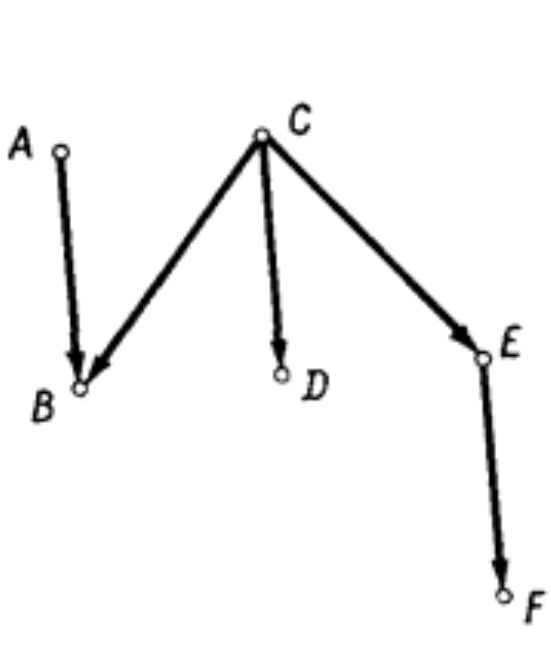
\includegraphics[scale=0.4]{рис1.jpg}
    \captionof{figure}{}
\end{minipage}
\begin{minipage}{0.2\textwidth} 
    \raisebox{-2cm}{
        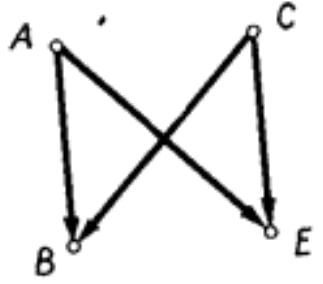
\includegraphics[scale=0.35]{рис2.jpg}
    }
    \captionof{figure}{}
\end{minipage}

Следующую (22-ю) партию проведем между \textit{B} и \textit{C}. Если победит \textit{B}, то ясно, что \textit{A} --- чемпион, \textit{B} --- второй призер, а на третье место претендуют пятеро, проигравших \textit{B}. За оставшиеся 4 партии можно найти среди них третьего призера. 

\switchcolumn

Пусть наоборот, победит \textit{C}. Тогда возникнет следующая ситуация (см. рис. 1): на призовые места претендуют шахматисты \textit{А}, \textit{В}, \textit{C}, \textit{D}, \textit{E} и \textit{F} (стрелки ведут от победителя к побежденным). Проверим 23-ю партию между \textit{D} и \textit{E}; пусть в этой партии победит \textit{E} (случай, когда победит \textit{D}, проще и рассматривается аналогично).

24-ю партию проведем между \textit{А} и \textit{Е}. Если выиграет \textit{Е}, то \textit{С} --- чемпион, \textit{Е} --- второй призер, а на третье место претендуют \textit{А}, \textit{D} и \textit{F}. За оставшиеся 2 партии найдём среди них третьего призера.

Если 24-ю партию выиграет \textit{А}, то (см. рис. 2) на первые два места претендуют \textit{А} и \textit{С}, на третье --- \textit{В} и \textit{Е}. Проведя две партии (между \textit{А} и \textit{С} и между \textit{В} и \textit{Е}), мы определим 1-го, 2-го и 3-го призеров. Итак, $I \ (20)=26=P \ (20)$.

Только что приведенные правила резко отличаются от стандартных правил из главы III. По стандартным правилам шахматисты, проигравшие хоть одну партию , не участвуют в следующих играх до тех пор, пока не определится чемпион. Только отказавашись от этого , нам удалось определить 1-го, 2-го и 3-го призеров среди 20 шахматистов за 26 (а не за 27) партий.

\textbf{2}. Доказать, что 1-го и 2-го призеров среди \textit{n} шахматистов наверняка можно определить за $l \ [n] + n - 2$ партий и может не удаться определить за меньшее число партий.

\textbf{3}. Пусть мы хотим определить среди \textit{n} шахматистов \textit{k} сильнейших (1-го, 2-го, .., \textit{k}-го призеров). Докажите, что 

а) это наверняка можно сделать за $(k - 1) \ l \ [n] + n - k$ партий;

б) если
\[
R<l \ [n(n-1)\dots(n-k+2)]+n-k
\]
то результаты партий могут оказаться такими, что это не удается сделать за \textit{R} партий.

\so{Указание}. В задаче б) мы рекомендуем расуждать так же, как в главе II, рассматривая «команды» $A_1, A_2,\dots, A_{k-1}$, состоящие из k-1 участника. Общее число таких команд равно $n(n-1)\dots(n-k+2)$
}
\end{paracol}